\chapter[Direct method physics]{The physics of the Direct $T_e$ method}\label{sec:physics}

The Direct $T_e$ method is used to calculate the gas-phase chemical abundances 
(oxygen, nitrogen, etc. relative to hydrogen) in \ion{H}{2} regions.  It differs 
from other commonly-used methods by estimating the gas temperature and electron 
density of the region directly from the galaxy's spectrum.  UV photons from 
young stars in an \ion{H}{2} region keep the interstellar gas partially ionized.  
In an \ion{H}{2} region, a photon with an energy 
$E_\gamma \gtrsim 13.6\text{ eV}$ ionizes a hydrogen atom, producing an H$^+$ 
ion and an electron with some kinetic energy 
$K_{e^-} = E_\gamma - 13.6\text{ eV}$.  As the free electron moves around in the 
gas, it loses some of its kinetic energy as it collisionally excites other ions 
in the gas.  Because we are in a Str\"{o}mgren sphere (an ionized region or an 
\ion{H}{2} region), the cross-section for this electron scattering is much 
larger than the photoionization cross section, so the free electrons will 
thermalize quickly \citep{DeRobertis87}.  Eventually, the free electron 
recombines with an H$^+$ ion, forming atomic hydrogen.  The ions that are 
collisionally excited by the electron before its recombination eventually 
de-excite via forbidden transitions, emitting radiation that escapes the 
\ion{H}{2} region.

In equilibrium, the total energy input into the gas via radiation from the star 
(that ionizes the hydrogen), $E_{photoionization}$, must be equal to the energy 
required to recombine the electron and the H$^+$ ion, $E_{recombination}$, and 
the energy radiated away from the \ion{H}{2} region by the forbidden 
transitions, $E_{radiation}$.  So
\begin{equation}
    E_{photoionization} = E_{recombination} + E_{radiation}
\end{equation}
For radiative de-excitation to dominate over collisional de-excitation, the 
electron density $n_e \ll 10^{8-10}\text{ cm}^{-3}$ \citep{DeRobertis87}.  
Typical \ion{H}{2} regions have an electron density 
$n_e \approx 100\text{ cm}^{-3}$, so radiative de-excitation dominates; this is 
why we observe forbidden transitions in outer space but not here on Earth.


\section{Forbidden transitions}

Similar to a fingerprint, every element has a unique set of wavelengths seen in 
its spectrum that corresponds to the atom's different energy levels.  Since 
electrons within an atom have discrete energy levels, transitions between levels 
result in either the emission (when decreasing in energy) or absorption 
(an increase in energy) of a photon of the same energy as the difference between 
the two levels.  The separation between energy levels is unique for each 
element, so the photon energies either emitted or absorbed by each element are 
unique.


\subsection{Time-dependent perturbation theory}

A time-dependent potential is added to the Schr\"{o}dinger equation in order to 
solve for the forbidden transition energies.  We can assume that the time 
perturbation is a minor component of the potential and can thus treat it as a 
perturbation.  For a simplified two-level system, the time-dependent wave 
function is
\begin{equation}
    \Psi (t) = c_a (t) \psi_a e^{iE_a t/\hbar} + c_b (t) \psi (b) e^{-iE_b t/\hbar}
\end{equation}
To solve for the time-dependent coefficients, we substitute $\Psi (t)$ into the 
time-dependent Schr\"{o}dinter equation
\begin{equation}
    H\Psi = i\hbar \frac{\partial \Psi}{\partial t}, \qquad \text{where } H = H^0 + H'(t)
\end{equation}
We find that
\begin{align}
    \dot{c}_a &= -\frac{i}{\hbar} H'_{ab} e^{-i\omega_0 t} c_b\\
    \dot{c}_b &= -\frac{i}{\hbar} H'_{ba} e^{-i\omega_0 t} c_a
\end{align}
where
\begin{equation}
    \omega_0 \equiv \frac{E_b - E_a}{\hbar}
\end{equation}
and
\begin{equation}
    H_{ij} \equiv \langle \psi_i | H' | \psi_j \rangle
\end{equation}
The probability that transmission has occurred is $P_{b\to a} = |c_a (t)|^2$.  
The transmission rate $R_{a\to b} = dP/dt$.

For an electromagnetic wave, the atom experiences an oscillating electric field.  
For visible light, it is typically safe to assume that the spatial portion of 
the field does not change, since the wavelength is much longer than the size of 
the atom.  However, if we consider a spatial variation of the field, we find 
that the true electric field is
\begin{equation}
    \vec{E}(\vec{r},t) = \vec{E}_0 \cos (\vec{k}\cdot \vec{r} - \omega t)
\end{equation}
Expanding this to first order, we find that
\begin{equation}
    \vec{E}(\vec{r},t) = \vec{E}_0 [\cos (\omega t) + (\vec{k} \cdot \vec{r} \sin (\omega t)]
\end{equation}
The first term in this approximation represents the electric dipole transitions 
(the canonical electron transitions).  The second term leads to forbidden 
transitions (magnetic dipole and electric quadrupole).
%This oscillating field corresponds to our perturbing Hamiltonian:
%\begin{equation}
%    H' = -qE_0 z\cos (\omega t)
%\end{equation}
%where $q$ is the charge on the electron, and the electric field is oscillating 
%in the $z$ direction.  Thus,
%\begin{equation}
%    H'_{ba} = -pE_0 \cos (\omega t), \qquad \text{where } p \equiv q \langle \psi_b |z| \psi_a \rangle
%\end{equation}


%\subsection{Forbidden transitions --- metastable energy levels}




%\subsection{Selection rules}
%
%The transmission rates depend on a matrix element of the form 
%$\langle \psi_b |\vec{r}| \psi_a \rangle$.  Denoting the states by the quantum 
%numbers $n$, $l$, and $m$, the matrix elements can be written as
%\begin{equation}\label{eq:matrix_elements}
%    \langle n'l'm' |\vec{r}| nlm \rangle
%\end{equation}
%By applying the various angular momentum commutators \citep[as shown in][]
%{Griffiths05}, we can develop a set of selection rules for allowed transitions 
%of the electron in an atom.
%
%Inserting the commutation relation $[L_z, z] = 0$ into Eqn. 
%\ref{eq:matrix_elements}, we find that
%\begin{align}
%    0 &= \langle n'l'm'|[L_z, z]|nlm \rangle\\
%    &= \langle n'l'm'|(L_z z - zL_z)|nlm \rangle\\
%    &= \langle n'l'm'|(m'\hbar)z - z(m\hbar)|nlm \rangle\\
%    0 &= (m' - m)\hbar \langle n'l'm'|z|nlm \rangle
%\end{align}
%$\langle n'l'm'|z|nlm \rangle = 0$ is a boring result, so we find that
%\begin{equation}\label{eq:m'=m}
%    m' = m
%\end{equation}
%
%Likewise, by employing the relation $[L_z, x] = i\hbar y$, we find that
%\begin{equation}\label{eq:Lz_x}
%    (m' - m)\hbar \langle n'l'm'|x|nlm \rangle = i\hbar \langle n'l'm'|y|nlm \rangle
%\end{equation}
%With the relation $[L_z, y] = -i\hbar x$, we find that
%\begin{equation}\label{eq:Lz_y}
%    (m' - m)\hbar \langle n'l'm'|y|nlm \rangle = -i\hbar \langle n'l'm'|x|nlm \rangle
%\end{equation}
%Combining Eqns. \ref{eq:Lz_x} and \ref{eq:Lz_y} (and again, ignoring the boring 
%result), we find that
%\begin{equation}\label{eq:m'=+/-m}
%    (m' - m)^2 = 1
%\end{equation}
%Eqns. \ref{eq:m'=m} and \ref{eq:m'=+/-m} show that transitions will only occur 
%if $\Delta m = \pm 1,0$.






\section[Estimating the temperature]{Temperatures from the forbidden emission lines}

%%%%%%%% All from DeRobertis87
%Of the ions that dominate radiative cooling (O$^+$, N$^+$, etc.), most have 
%either p$^2$, p$^3$, or p$^4$ ground-state electron configurations with five 
%energy levels $\leq 5\text{ eV}$ above the ground state.  For each excitation 
%level $i$, \cite{DeRobertis87} shows that the equations of statistical 
%equilibrium are
%\begin{equation}
%    \sum_{j \neq i} n_j n_e q_{ij} + \sum_{j > i} n_j A_{ji} = \sum_{j \neq i} n_i n_e q_{ij} + \sum_{j < i} n_i A_{ij}
%\end{equation}
%where $n_j$ is the fraction of the ion in level $j$, $q_{ij}$ is the electron 
%(de)excitation rate coefficient (in units of cm$^{-3}$s$^{-1}$), and $A_{ij}$ is 
%the radiate transition probability with units of s$^{-1}$.  From left to right, 
%these terms describe the collisional transitions to $i$, the radiative 
%transitions down to $i$, the collisional transitions from $i$, and the radiative 
%transitions down from $i$.  For a given ion X$^i$ with a number density 
%$N(\text{X}^i)$, the relative populations must must sum to unity:
%\begin{equation}
%    \sum_j \frac{n_j}{N(\text{X}^i} = 1
%\end{equation}
%
%$A_{ij}$ are independent of temperature and inversely proportional to the 
%lifetime of the upper level.  Conversely, the coefficients $q_{ij}$ depend on 
%temperature since they are a measure of how likely collisions will occur.  These 
%can be calculated as
%\begin{equation}
%    q_{ij} = \frac{8.629\times 10^{-6}}{T_e^{1/2}} \frac{\Omega (i,j)}{\omega_i}
%\end{equation}
%where $T_e$ is the electron temperature, $\omega_i$ is the statistical weight of 
%level $i$, and $\Omega (i,j)$ is the average collisional strength.  While 
%$\Omega$ is dimensionless, it does depend on the temperature 
%\cite{DeRobertis87}.  The excitation rate $q_{ij}$ is related to the 
%de-excitation rate $q_{ji$ by
%\begin{equation}
%    q_{ji} = \frac{\omega_i}{\omega_j} q_{ij} \exp{-\Chi_{ij}/kT}
%\end{equation}
%where $\Chi_{ij}$ is the excitation energy difference between levels $i$ and 
%$j$.


%%%%%%% From Osterbrock89

%In a pure hydrogen nebula, \cite{Osterbrock89} shows us that the photoionization 
%energy input (per unit volume per unit time) is equal to 
%\begin{equation}
%    G(H) = n_e n_p \alpha_A (H^0, T) \frac{3}{2} kT_i
%\end{equation}
%where $n_e$ is the number density of electrons, $n_p$ is the number density of 
%protons, $\alpha_A$ is the recombination coefficient summed over all energy 
%levels, and $T_i$ is the photoelectron's initial temperature.  Assuming a 
%blackbody spectrum, $T_i \approx T_*$ for $kT_* < h\nu_0$.  The gain $G(H)$ 
%depends on the form of the ionizing radiation field, not its strength.  The rate 
%of creation of the photoelectrons depends on the strength of the radiation 
%field, or the recombination rate.
%
%Likewise, \cite{Osterbrock89} shows that the rate of energy lost through 
%recombination per unit volume is equal to
%\begin{equation}
%    L_R (H) = n_e n_p kT \beta_A (H^0, T)
%\end{equation}
%where $\beta_A$ is the effective recombination coefficient for recombination 
%energy loss.

Expanding the description in Sec. \ref{sec:O3}, we can define the ratio of the 
emission line strengths for [\ion{O}{3}] $\lambda$4363 and [\ion{O}{3}] 
$\lambda \lambda$4959,5007 as
\begin{equation}
    \frac{j_{4959} + j_{5007}}{j_{4363}} = \frac{\Omega(^3\text{P}, ^1\text{D})}{\Omega(^3\text{P}, ^1\text{S})} \left[ \frac{A_{^1\text{S}, ^1\text{D}} + A_{^1\text{S}, ^3\text{P}}}{A_{^1\text{S}, ^1\text{D}}} \right] \frac{\bar{\nu}(^3\text{P}, ^1\text{D})}{\nu(^1\text{D}, ^1\text{S})} e^{\Delta E/kT}
\end{equation}
where
\begin{equation}
    \bar{\nu}(^3\text{P}, ^1\text{D}) = \frac{A_{^1\text{D}_2, ^3\text{P}_2}\nu (\lambda 5007) + A_{^1\text{D}_2, ^3\text{P}_1}\nu (\lambda 4959)}{A_{^1\text{D}_2, ^3\text{P}_2} + A_{^1\text{D}_2, ^3\text{P}_1}}
\end{equation}
and $j_\lambda$ is the emissivity of the emission line, $\Omega (i,j)$ is the 
collision strength between levels $i$ and $j$, $A_{i,j}$ is the radiative 
transition probability between an upper level $i$ and a lower level $j$, $\nu$ 
is the frequency of the transition, $\Delta E$ is the energy difference between 
the $^1$D$_2$ and $^1$S$_0$ levels, and $T$ is the electron temperature 
\citep{Osterbrock89}.  The transition probabilities $A_{i,j}$ do not depend on 
the temperature, but the collision strength $\Omega (i,j)$ is 
temperature-dependent.  We can define
\begin{equation}
    \bar{\nu}(^3\text{P}, ^1\text{D}) = \frac{A_{^1\text{D}_2, ^3\text{P}_2} \nu (5007) + A_{^1\text{D}_2, ^3\text{P}_1} \nu (4959)}{A_{^1\text{D}_2, ^3\text{P}_2} + A_{^1\text{D}_2, ^3\text{P}_1}}
\end{equation}
Inserting numerical values for the collision strengths and transition 
probabilities from \cite{Osterbrock89}, the ratio becomes
\begin{equation}
    \frac{j_{4959} + j_{5007}}{j_{4363}} = \frac{7.73 \exp[(3.29\times 10^4)/T]}{1 + 4.5\times 10^{-4} (N_e/T^{1/2})}
\end{equation}
Fig. \ref{fig:OIII_temp} shows how this ratio depends on the temperature.  By 
measuring the flux of these emission lines, we can then solve for the 
temperature of the gas.

\begin{figure}
    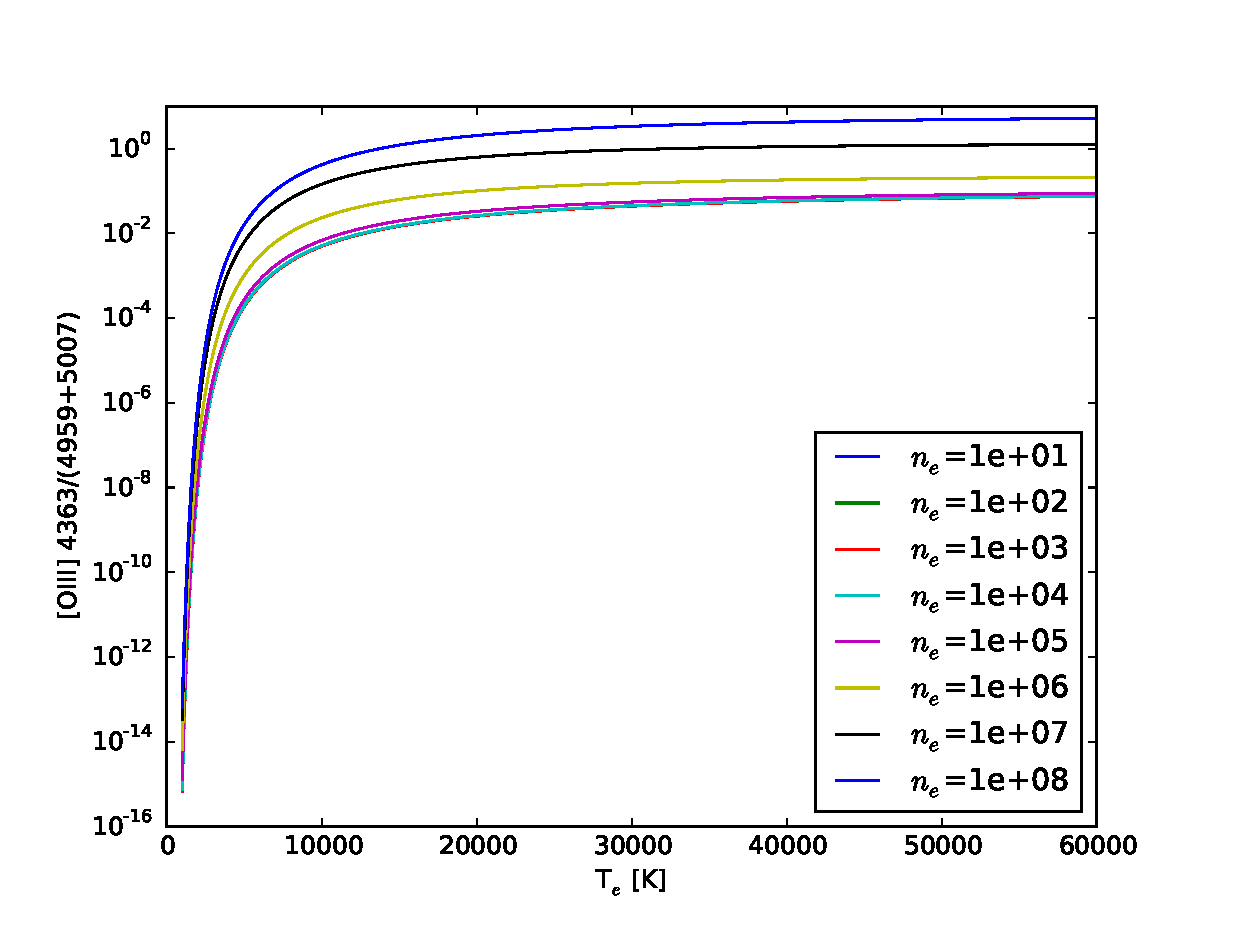
\includegraphics[width=0.75\textwidth]{Images/Appendix/[OIII]}
    \caption[{[\ion{O}{3}] ratio as a function of temperature}]{The [\ion{O}{3}] 
    $\lambda$4363/($\lambda$4959 + $\lambda$5007) ratio as a function of 
    temperature for various densities \citep{Luridiana15}.  Typical electron 
    densities in \ion{H}{2} regions are $\sim$100 cm$^{-3}$.}
    \label{fig:OIII_temp}
\end{figure}


\section{[\ion{S}{2}]}

Similar to the sensitivity of the doubly-ionized oxygen ion transitions to the 
electron temperature of the surrounding gas, the transitions for singly-ionized 
sulfur are sensitive to electron number density.  The relative excitation rates 
depend only on the ratio of the collision strengths when two emission lines 
(from the same ion) with nearly identical excitation energies are compared 
\citep{Osterbrock89}.  If the two levels have different transition probabilities 
and/or different collisional de-excitation rates, their ratio depends on the 
density.

The relative excitation rates of the two lines shown in Fig. 
\ref{fig:transitions_P1} are proportional to their statistical weights; thus, the 
ratio of the line intensities is a constant in the low-density limit 
\citep{Osterbrock89}.  In the high-density regime, this ratio is best accurately 
described by a Boltzmann population ratio.  There is a critical density for the 
energy levels which describes the turning point between these two extremes.  A 
graphical representation of this ratio as a function of density can be seen in 
Fig. \ref{fig:SII_den}.  \ion{H}{2} regions typically have densities well within 
the low-density regime, so we set the electron density for all our galaxies at 
100 cm$^{-3}$.

\begin{figure}
    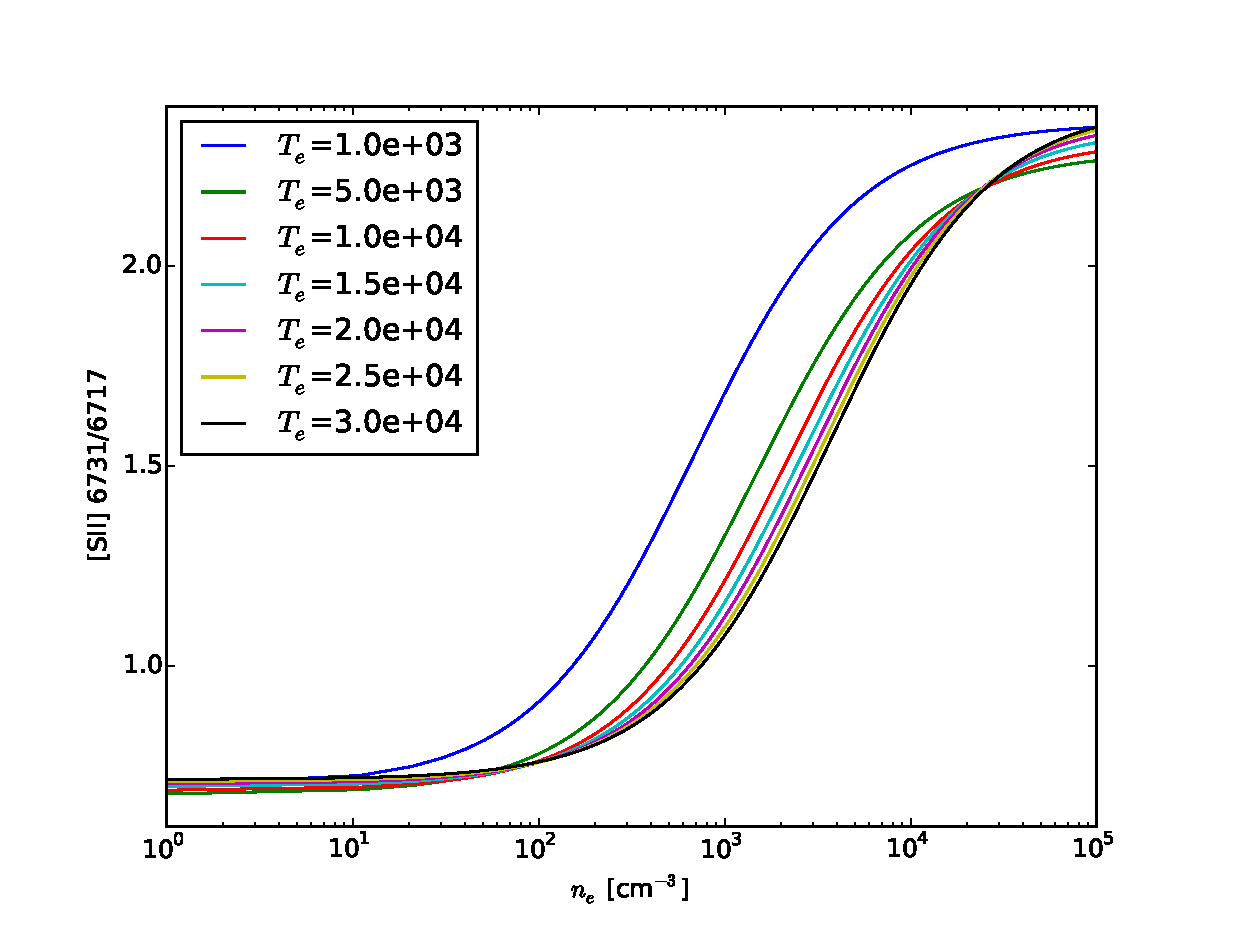
\includegraphics[width=0.75\textwidth]{Images/Appendix/[SII]}
    \caption[{[\ion{S}{2}] ratio as a function of density}]{The [\ion{S}{2}] 
    $\lambda$6731/$\lambda$6717 ratio as a function of density for various 
    temperatures \citep{Luridiana15}.  The gas temperatures of \ion{H}{2} 
    regions are typically around 10$^4$ K.}
    \label{fig:SII_den}
\end{figure}